% Előzmények (irodalomkutatás, hasonló alkotások), az ezekből levonható következtetések

% előző scriptek
% hivatalos programok is csak griden
% hol használnak még ilyet nyomtatáson kívül (üveg)
% ládapakolás, np nehéz
% extra megkötés, vágóasztallal vágás
% talált irodalom
% felhasznált pszeudokód? idk
% egyéb algoritmusok a strip packingen kívül

\chapter{Előzmények}

\section{Hivatalos szoftverek}

A Canon imagePROGRAF PRO-4600 plotterhez több különféle nyomtatási segédprogramot is kaptunk. Megpróbáltunk áttérni a használatukra, viszont alapvető funckiók hiányoztak belőlük. A legtöbb program csak kézzel való elrendezést tett lehetővé, a mi esetünkben ez viszont egy visszalépést jelentett volna a szkripttel szemben.

\section{A Photoshop szkriptről}

A szkript által használt algoritmus felettébb egyszerű. A dokumentumot egy rács mentén cellákra osztjuk fel, ahol minden cella mérete a kinyomtatni kívánt kép méretének felel meg.
Nem mindegy, hogy a cellák fekvő vagy álló tájolással vannak elhelyezve a dokumentumon, ugyanis ez különböző mennyiségű felesleget eredményezhet.

\begin{figure}[!h]
    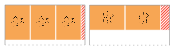
\includegraphics[width=\textwidth]{figures/wastecalc.pdf}
    \caption{Soronként keletkező felesleg eltérő tájolások mellett}
    \label{fig:wastecalc}
\end{figure}

Az orientáció kiszámításához megvizsgáljuk mindkét esetet, egy teljesen kitöltött sorra. Legyen a tekercs szélessége $W$, a keletkező felesleg pedig $A$. Vegyünk egy képet, ahol a kép szélessége $w$, magassága $h$, orientációja $r$. Ekkor a keletkező felesleg

$$m_1 = \bigg\lfloor \cfrac{W}{w} \bigg\rfloor, \qquad A_1 = (W - m_1 * w) * h,$$

\noindent illetve ellentétes orientáció esetén

$$m_2 = \bigg\lfloor \cfrac{W}{h} \bigg\rfloor, \qquad A_2 = (W - m_2 * h) * w.$$


A kevesebb felesleget eredényező eset határozza meg az orientációt. Az orientáció alapján kiszámolható az rács oszlopainak száma, $m$. Ez $n$ kinyomtatni kívánt kép esetén $k$ oszlopot eredményez, ahol

$$k = \bigg\lceil \cfrac{n}{m} \bigg\rceil.$$

\noindent Amennyiben

$$ n \mod m \neq 0,$$

\noindent úgy ez az eljárás üres cellákhoz, azaz papírfelesleghez fog vezetni. 

Emiatt született meg az opció a mennyiség korrigálására, mely megnöveli $n$-t úgy, hogy a korrigálás előtti esetleges üres cellákba is kerüljenek képek:

$$n' = k * m.$$

\begin{figure}[!h]
    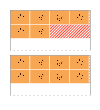
\includegraphics[width=\textwidth]{figures/correct_quantity.pdf}
    \caption{A mennyiség korrigálás}
    \label{fig:correct_quantity}
\end{figure}

Ez a megoldás sajnos nem tökéletes. Ha az utolsó sorunk cellái nincsenek teljesen kitöltve, akkor nem biztos, hogy $r$ orientáció valóban kevesebb felesleggel fog járni.

TODO még magyarázat hogy ezt hogyan vagy hogy erre még visszatérek idk

\section{Különböző méretű képek elrendezése}

A különböző méretű dobozok fix területre történő elhelyezése a ládapakolási problémára vezethető vissza. A mi problémánk egy speciális esete ennek. A tekercs szélessége fix, a magassága viszont tetszőleges, de minimalizálni szeretnénk. Az eredménynek vágóasztallal vághatónak kell lennie.

\subsection{Guillotine vágás}

A guillotine vágás egy olyan folyamat, ahol egy nagyobb lemezt vágunk fel előre megadott, kisebb téglalapokra, guillotine vágásokkal. A guillotine vágások, más néven széltől-szélig vágások egyik oldaltól a másik oldalig tartó egyenes vágások, melyek az téglalapot két részre osztják fel. Ezt az eljárást elsősorban üveg, acél, fa illetve kartonpapír lapok felvágásakor alkalmazzák. Több különböző szempont alapján is próbálhatjuk optimalizálni a problémát, például maximalizálni a kapott elemek területét, értékét vagy számát illetve minimalizálni a szükséges vágások számát vagy a keletkező felseleget.

A guillotine vágás esetén a lemezek mérete előre meg van adva, és a kisebb téglalapok mennyisége nincsen megkötve. A mi esetünk ugyan nagyban hasonlít a guillotine vágásra, leszámítva, hogy a képek mennyisége fix, és csak a tekercs szélessége adott. Ennek tudatában folytattuk tovább a kutatómunkát barátommal és kollégámmal, Orbán Levente Lászlóval.

% TODO forrás megjelölés: https://en.wikipedia.org/wiki/Guillotine_cutting

\subsection{Tekercsre pakolás probléma}

A tekercsre pakolás probléma egy két dimenziós geometriai minimalizálási probléma. Adott egy tekercs fix szélességgel és tetszőleges magassággal, valamint a tekercsre helyezendő téglalapok. Meghatározandó egy elrendezés, mely átfedés nélkül helyezi el a téglalapokat a tekercsre, minimalizálva a felhasznált tekercsrész magasságát. Legtöbbet a textil- és papírtekercsek feldolgozásával foglalkozó kontextusokban találkozhatunk ilyen megoldásokkal.

Sajnos a tekercsre pakolási probléma erősen NP-nehéz, mert magában tartalmazza a ládapakolási problémát fix magasságú elemekkel. 

% TODO forrás megjelölés: https://en.wikipedia.org/wiki/Strip_packing_problem

A feladatunk tehát visszavezethető a tekercsre pakolás és a guillotine vágás keveréke, egy tekercsre kell guillotine-nal vágható elrendezésben pakolnunk az elemeinket. Szerencsénkre ez már egy ismert speciális esete a tekercsre pakolásnak, és több különféle algoritmus is létezik már rá.

\section{A választott algoritmusok}

Egyetlen méret nyomtatása esetén a régi szkript kapcsán ismertetett rácsra helyezés javított változata már egy optimális megoldás, és megvan az opciónk, hogy korrigáljuk a mennyiséget az esetleges ki nem töltött cellák alapján. 

Különböző méretű képek esetén a probléma erősen NP-nehéz voltából adódóan úgy döntöttünk, hogy nem fogunk optimális megoldást keresni, ugyanis fontos szempont volt a program futásának ideje, és mert az esetek túlnyomó többségében nem nyomtatunk több különböző méretben egyszerre.  

Leventének köszönhetően találtuk meg a \cite{ph} cikket, melyben pont egy számunkra kedvező heurisztikus megoldást mutatnak be. Az algoritmus heurisztikus voltából adódóan nem ad mindig optimális megolást, komplexitása azonban csupán $O(n^2)$. A megoldás egy rekurzív megközelítést alkalmaz, ami elősegíti, hogy az eredmény biztosan vágóasztallal vágható legyen. A koncepció egyszerű: egy téglalapra helyezzük az elemeinket, minden lehelyezett elem további téglalapokat határoz meg. Egy elem elhelyezésénél öt esetet különböztethetünk meg.

\begin{figure}[!h]
    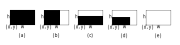
\includegraphics[width=\textwidth]{figures/priority.pdf}
    \caption{A lehetséges esetek egy elem elehelyezésekor. A fekete téglalapok az elemet jelölik.}
    \label{fig:placements}
\end{figure}

Az \href{fig:placements}{(a)} eset a legkedvezőbb, ebben az esetben a rendelkezésre álló helyet az elem teljesen kitölti. A \href{fig:placements}{(b)} és \href{fig:placements}{(c)} esetek kedvezőbbek, mint \href{fig:placements}{(d)}, mert ekkor az üresen maradt hely egyetlen téglalapot eredményez. Az \href{fig:placements}{(e)} esetben semmilyen elemet sem tudunk a téglalapra helyezni, a terület ekkor felesleggé válik.

Első lépésben minden elemünket a rövidebbik élére állítjuk, majd valamilyen heurisztika alapján sorba rendezzük őket (pl. magasság szerint csökkenő sorrendbe). Az ábra (\ref{fig:placements}) alapján \href{fig:placements}{(a)}-\href{fig:placements}{(e)} esetekhez rendre prioritásokat rendelünk, ahol \href{fig:placements}{(a)} prioritása a legnagyobb. 
Meghatározzuk a hátralevő elemeink prioritását, mind álló, mind fekvő helyzetben, és vesszük a legnagyobb prioritásút, feljegyezve annak orientációját. Ha két elemnek megegyezik a prioritása, a sorba rendezésbeli helyük alapján a sorban előrébb lévő elemet vesszük, azon belül pedig a fekvő tájolású elemet részesítjük előnyben.

Az így kapott elemet az feljegyzett orientációban a téglalapra helyezzük. A \href{fig:placements}{(d)} esetben nem mindegy, hogy hogyan osztjuk tovább a téglalapot. A hátralevő elemeink közül megkeressük a legrövidebb előforduló oldal hosszát, legyen ez $s_\text{min}$. 

\begin{figure}[!h]
    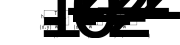
\includegraphics[width=\textwidth]{figures/partitioning.pdf}
    \caption{A téglalap lehetséges felosztása}
    \label{fig:partitioning}
\end{figure}

Az ábra (\ref{fig:partitioning}) alapján amennyiben $w - s_1 < s_\text{min}$, úgy \href{fig:partitioning}{(d\textsubscript{1})} szerint osztjuk fel, mert ekkor T\textsubscript{2} téglalapra egyik esetben sem fér el egyik elem sem, azaz ez a rész felesleggé válik, vagyis azt az esetet választjuk, ahol ez kisebb. Hasonlóképpen ha $h - s_2 < s_\text{min}$, akkor \href{fig:partitioning}{(d\textsubscript{2})} szerint osztjuk fel a téglalapot, és T\textsubscript{1} lesz a felesleg. Amennyiben egyik feltétel sem teljesül, úgy kétféleképp is feloszthatjuk a téglalapot. A felosztást $s_1 < s_\text{min}$ feltétel határozza meg: ha teljesül, akkor \href{fig:partitioning}{(d\textsubscript{1})} esetet választjuk, mert ellenkező esetben T\textsubscript{1} felesleggé válna.

A keletkező üres téglalapokra újból meghatározzuk a hátralevő elemek prioritásait és rekurzívan folytatjuk a pakolást, amíg el nem helyeztünk minden elemet, vagy már nincsen téglalap, amire elemeket tudnánk helyezni.

Adott elemekre más-más sorba rendezési heurisztikák más-más elrendezéseket eredményeznek, ezért nem mindegy, hogy hogyan választjuk meg. Az elemhalmazunktól nagyban függ, hogy éppen milyen szempont alapján érdemes őket sorba rendeznünk, de ezt nehéz előre meghatározni. Érdemes az algoritmust több különböző sorba rendezés szerint futtatni, és az eredmények közül a legkedvezőbbet választani. Ilyen rendezések lehetnek példálul magasság, terület, kerület, átló szerinti csökkenő sorrendek.

% TODO egyéb heurisztikák